\documentclass[11pt,letterpaper]{article}
\usepackage[top=1.00in, bottom=1.0in, left=1in, right=1.25in]{geometry}
\usepackage{graphicx}
\usepackage{latexsym,amssymb,epsf}
\usepackage{epstopdf}

\usepackage{sectsty,setspace,natbib}
\usepackage{float}
\usepackage[colorinlistoftodos,prependcaption,textsize=tiny]{todonotes}
\usepackage{latexsym}
\usepackage{epsfig}
\usepackage{graphicx}
\usepackage{amsmath}
\usepackage{array}
\usepackage{lineno}
\usepackage{gensymb}
\usepackage{xr-hyper}
\externaldocument{phenncc_supp}
% \externaldocument{letters/phencc/revision2/phencc_ELE_revletter2_p2}
% \usepackage{hyperref}
\newcommand{\R}[1]{\label{}\linelabel{#1}} % \newcommand{\R}[1]{\label{#1}\linelabel{#1}}
\newcommand{\lr}[1]{line~\lineref{#1}}

\usepackage{framed}

\linespread{1.1} % was 1.66 for double-spaced 
% \raggedright
\setlength{\parindent}{0.5in}
\pagestyle{empty}

\parskip=5pt
\pagenumbering{arabic}
\pagestyle{plain}
\setlength\parindent{0pt}

\begin{document}
\begin{flushright}
Version dated: \today
\end{flushright}
\bigskip
\noindent Running head: Tracking \& climate change
% put in your own RH (running head)
\bigskip
\medskip
\begin{center}
% Insert your title:
\noindent{\Large {\bf How phenological tracking shapes species and communities \\in non-stationary environments}}\\
% Other titles: `Environmental tracking: It's more complicated than you think' (we hope) 
% or `Environmental tracking: Is it naive? Or, are we just naive?'
\bigskip
\noindent {\normalsize
E. M. Wolkovich$^{1}$ \& M. J. Donahue$^{2}$ }\\
\noindent {\small \it
$^1$ Forest \& Conservation Sciences, Faculty of Forestry, University of British Columbia, 2424 Main Mall, Vancouver, BC V6T 1Z4 (e.wolkovich@ubc.ca)\\
$^2$ Hawai`i Institute of Marine Biology, University of Hawai`i at M\= anoa, K\=an`eohe, HI 96744 (donahuem@hawaii.edu)}\\
\medskip
\end{center}
\noindent{\bf Corresponding author:} see$^{1}$ above; Ph: 604.827.5246 (no fax).\\

\noindent \emph{Authorship statement:} EMW and MJD both conceived of the paper, produced the figures, performed modeling work and edited the paper, EMW wrote the paper and did the literature review, while MJD wrote the supplementary information on the model.  \\
% \noindent \emph{Data statement:} Review, so no new primary data, but data from a comprehensive literature review will be archived in an appropriate public repository and the data DOI will be included at the end of the article. \\
\noindent \emph{Keywords:} community assembly, global change, climate change, phenology, environmental variability\\
\noindent \emph{Article information:} Abstract: 217 words; Main text: 7410; Figures: 6; 119 references

% https://onlinelibrary.wiley.com/page/journal/1469185x/homepage/forauthors.html

\newpage
\begin{abstract} 
% 217 words
Climate change reshapes the environments of all species. Predicting species responses requires understanding how well species can track environmental change, and how such tracking shapes communities. Growing empirical evidence suggests that how species track environmental change phenologically---how an organism shifts the timing of major biological events in response to the environment---is linked to species performance and is a structuring force of species and communities today. Such research tantalizingly suggests a potential framework to predict the winners and losers of climate change, and the future communities we can expect. But developing this framework requires far greater efforts to ground empirical studies of phenological tracking in relevant ecological theory.

Here, we review the concept of tracking in empirical studies and through the lens of coexistence theory in community ecology. We argue that much current theory for tracking ignores the importance of a multi-species context beyond trophic interactions. Yet community assembly theory predicts competition should drive variation in tracking and trade-offs with other traits. Existing community assembly theory can help us understand tracking in stationary and non-stationary systems and, thus, predict the species- and community-level consequences of climate change. But it will require greater efforts to integrate priority effects into modern coexistence theory and improved empirical estimates of environmental change, phenological tracking and underlying environmental cues.  % We examine how coexistence theory can be extended to test the current paradigm that climate change should favor species with environmental tracking.
\end{abstract}
% Finally, we consider how the reality that climate change has widespread effects beyond mean temperature, including shifts in growing season length, variability, and in extreme events, may complicate simple predictions of winners and losers. 
% Limited understanding of organism's phenological cues combined with statistical issues may make many current estimates of variation in tracking less reliable than they appear. Yet these estimates provide the crucial first step to understand variation. 
\tableofcontents

\newpage
% \linenumbers % If you want to add need to add \begin{linenomath} and \end{linenomath} around all eqns (and check they still show up)
\section{Introduction}
Anthropogenic climate change is causing widespread changes in species distributions, with many species shifting in both time and space \citep{IPCC:2014sm,ipcc1point5}. Species are moving to higher elevations and poleward \citep{Chen2011}, shifting their recurring life history events (phenology) earlier \citep{Wolkovich:2012n,cohen2018}, or both as climate warms \citep{amano2014,socolar2017}. These general trends, however, hide high variability across species. A large proportion of species are not shifting \citep{Cook:2012pnas,amano2014}, which has raised concerns about whether these species may be more vulnerable to population declines with continued warming. Such concerns come in part from increasing research that links how well species track climate change by shifting their phenology to changes in biomass, growth and other metrics related to performance \citep{Cleland:2012}. Tracking may then be a major component to understanding and predicting the fitness consequences of climate change, including population declines, with cascading effects on community and ecosystem structure \citep{Menzel:2006xn,Parmesan:2006cr}. 

The hypothesis that tracking improves fitness outcomes with climate change has gained significant traction in the ecological literature \citep[e.g.,][]{Cleland:2012} and several areas of theory support it. Niche models of community assembly suggest that a warming climate should open up new temporal niche space and favor species that can exploit that space \citep{gotelli1996,wolkovich:2010fee,Zettlemoyer2019}.  However, there has been comparatively little work connecting tracking to community assembly theory. Yet theory shows temporal sequencing and environmental variability can alter the relative fitness and niche differences between species that determine coexistence---suggesting important ecological constraints to tracking. % Evolutionary models predict species that track will be favored in novel environmental conditions \citep{chevin2010}. 

%%''This disconnect'' has a vague antecedent.  Maybe:  `Predicting the fitness outcomes of tracking are complicated because most ecological theory was constructed for stationary systems.' Or `The outcomes of tracking under climate change depend on the nature of environmental variability - and most ecological theory was constructed for stationary systems. ... Lizzie says: I am okay with it, there are so many long sentences already, I hate to overload another
This disconnect could be because most ecological theory was constructed for stationary systems \citep[e.g.,][]{Chesson:1997dz}. While major arenas of research such as `modern coexistence theory' or population ecology now embrace environmental stochasticity, they generally still assume stationarity, where the underlying distribution of the environment is unchanged across time \citep[i.e., constant mean and variance,][]{barabas2018}.

Climate change upends the assumption of stationarity. By causing increases in temperature, larger pulses of precipitation, shifts in snowpack, increased drought, and more storms \citep{ipcc2013}, climate change has fundamentally shifted major attributes of the environment from stationary to non-stationary regimes (see Fig. \ref{fig:climdat}). This transition is reshaping ecological systems. New work has aimed to adapt coexistence theory to non-stationary environments \citep{chessonnonstat,volkerass}. Yet there is still little theoretical work on what such a transition may mean for communities and the species within them, including how community-level processes might feedback to modify species responses.

Here, we review the concept of phenological tracking as commonly used in the empirical climate change impacts literature and in related ecological theory. We begin by providing the necessary definitions to link empirical estimates to ecological theory: specifically we distinguish between measuring tracking in current environments and evaluating the fitness outcomes of tracking. After a brief review of current estimates of tracking, and basic theory that predicts variation in tracking across species and environments, we examine how well community assembly theory---especially priority effects and modern coexistence theory---can be extended to predict the community consequences of climate change. We close by reviewing the major hurdles to linking empirical estimates of phenological tracking and new ecological theory in the future. % test the current paradigm that climate change should favor species that track.  

\section{Defining \& measuring tracking}
\subsection{Phenological events}
Understanding the role of phenological tracking in community assembly first requires an understanding of phenological events. In empirical studies in climate change today, phenological events are often coded as on/off switches (e.g., a seed does/does not germinate; a coral does/does not spawn), yet these events are almost always defined by investment decisions that are part of a continuous developmental process \citep{chuinearees,inouye2019}---a critical distinction to help understand the forces that shape phenological tracking, and, in turn, how it may structure communities with climate change. 

Phenological events can be considered as the outcome of a two-part process that is repeatedly observed over time. At each temporal unit, an event can either happen or not (when---part 1) and, if it happens, the event can vary in size or degree of investment (how much---part 2). This process is generally applied at the level of the individual (but it could potentially apply at lower levels, for example buds on a branch, or potentially higher levels, such as all the offspring from a parent). Across time, it produces an event's distribution \citep{gotelli1996,steer2019}. After starting, many events are entrained to continue based on the underlying physiological process: for example, laying eggs within one clutch (here, the first part of the process is whether to lay eggs or not and the second is whether to continue to invest in that process, which would lead to additional eggs, which researchers then observe as number of eggs per temporal unit) or flowering each growing season. In such cases, first events at the individual-level are somewhat unique from the rest of the event's distribution. In all cases, these individual-level distributions scale up to the population-level estimates of these events generally used by researchers \citep[see][for discussion of the outcomes of this scaling]{inouye2019}. Variation in these events forms the basis of phenological tracking. 

\subsection{Defining tracking}
Tracking is a commonly used word in studies of how phenology is shifting with climate change \citep[e.g.,][]{Menzel:2006xn,Parmesan:2006cr,Cleland:2012,deacy2018}. Yet there are few, if any, definitions of it. Conceptual and theoretical treatments of tracking often relate how well an organism matches the timing of a life history event to the ideal timing for that event, what we refer to as `fundamental tracking.' In contrast, empirical studies of tracking often focus on estimating a change in the timing of an event relative to a measured environmental variable, with the aim of measuring what we refer to as `environmental tracking' (Fig. \ref{fig:defineETorig}-\ref{fig:defineET})---the phenological change due to an organism's cue system given change in the environment \citep[though most studies lack the required knowledge of the underlying cue system,][]{chmura2019}. 

Fundamental tracking rests on an assumption that there is a timing (an `ideal timing') that yields maximum fitness, and event timings moving away from this ideal result in reduced fitness \citep[a foundational concept of the trophic mismatch literature,][]{vissergienapp2019}. Yet this ideal timing is generally only clear in simplified models or in retrospect, thus species must use environmental cues to attempt to predict and match their phenology to the ideal timing across environments in both space and time (Fig. \ref{fig:defineETorig}-\ref{fig:defineET}); this match between ideal timing and actual timing is often referred to as cue reliability \citep{donald2013,bonamour2019}. Each organism's set of cues forms the biological basis for how a species tracks the environment.

An organism's cues combined with the environment's variability---which aspects of the environment vary, how (e.g., temporally each year, spatially at $x$ scale) and how much---determine what we refer to as `environmental tracking' (Fig. \ref{fig:defineET}, note the shift in timing between sites)---the phenological change due to an organism's cue system given change in the environment. While fundamental tracking forms the focus of most conceptual and theoretical treatments of phenological tracking, the majority of  empirical studies focus on estimating environmental tracking. 

Our definition of environmental tracking is sufficiently exact to be something that can be accurately modeled,  but its exactness also highlights the difficulty of measuring it. If the varying components of the environment are not in the organism's set of cues, then the organism does not `track' per this definition (although covariation with other environmental components might give the appearance of tracking).  Which aspect(s) of the environment researchers measure will determine their estimates of environmental tracking (e.g., a thermal threshold in Fig. \ref{fig:defineET}). If researchers know the exact cue or suite of cues (e.g., a interaction of thermal sums and daylength) and can perfectly measure these in an environment where the cue(s) varies, then an organism will track the environment perfectly. If researchers measure some related attribute (e.g., mean spring temperature in place of thermal sums) or only some of the organism's cues, then the organism will appear to track poorly (i.e., a noisier statistical relationship from poor measurement quality). Most empirical studies, however, lack the required knowledge of the underlying cue system \citep{chmura2019}, making most current estimates difficult to evaluate. %  (discussed below in section `Robust comparable measures of phenological tracking')

\iffalse
\subsection{Extras for now}
This is a foundational concept of the trophic mis-match literature \citep{vissergienapp2019}, which often assumes the peak timing of a resource defines the ideal timing for phenological events dependent on that resource \citep[e.g. egg laying dates dependent on caterpillar abundance,][]{Visser:2005bg}. For most events, however, fitness outcomes are likely dependent on a suite of interacting forces \citep[e.g.,][]{reed2013}---for example, egg laying dates for migratory birds may depend both on the timing of peak prey abundance and the need to leave nesting grounds before winter. Additionally, the timing of events is often connected to the investment process of an event \citep[e.g., number of eggs in a clutch,][]{inouye2019} in current, and sometimes past and future, years. Whatever their full underlying causes, fitness consequences of suboptimal timing should favor the evolution of organismal cues to predict and match the optimal timing (the degree of this match defines cue reliability, Fig. \ref{fig:defineET}). 

Environmental tracking at the individual-level is a purely plastic response to environmental variation \citep[in line with current findings on most climate change responses,][]{bonamour2019}, with the plasticity itself an outcome of selection \citep{chevin2010} through its connection to fundamental tracking (Fig. \ref{fig:defineETorig}). At the population-level, tracking may also incorporate evolutionary change---change in genotype frequencies---depending on both the timescales of study and the species' generation time \citep[this evolutionary response can be predicted as the difference between the environmental sensitivity of phenotypic selection and an organism's plasticity, $|B-b|$ in][]{chevin2010}. 
\fi

\subsection{Measuring tracking}
Measuring `tracking' and comparing variation in it across species, space and time is a rapidly growing area of ecological research \citep[e.g.,][]{Cook:2012pnas,fu2015,thackeray2016,cohen2018}. Studies that directly quantify fundamental tracking are uncommon \citep[but see][]{visser2006,charm2008}, given in part the difficulty of estimating fitness, though many studies in the synchrony literature attempt to link consumer change to resource change, with an assumption that the measured resource is the dominant determinant of ideal timing for the consumer \citep[though this may rarely be true, see][]{Singer:2010eb,Johansson2012,reed2013}. Instead, most studies focus on estimates closer to environmental tracking. Some studies estimate simply change in days over time \citep[e.g.,][]{Parmesan:2007tv,kharouba2018}, though most studies now estimate shifts as responses per unit temperature \citep[for example, multiple meta-analyses show plants' spring phenology shifts with spring or annual temperatures 4-6 days/$\degree$C on average across species,][]{Richardson:2006qh,Wolkovich:2012n,thackeray2016} or precipitation \citep{inouye2002,Craine:2012kl}. % In many studies environmental tracking is estimated as the slope of phenological event dates regressed against environmental metrics hypothesized to link to underlying cues, though this estimate will be more or less accurate depending statistical limitations and current knowledge of an organism's cue(s) \citep{chmura2019}.

All species-rich studies of phenology-climate relationships find high variation \citep{Cook:2012pnas,thackeray2016}, including some species that do not track or track poorly (i.e., high noise surrounding observed statistical relationships). Researchers have worked to link such variation to the underlying cues \citep[e.g.,][]{Cook:2012pnas}, species traits \citep[e.g.,][]{cohen2018} and trophic level \citep[e.g.,][]{thackeray2016}. These approaches hint at the three majors explanations for why some species do not appear to track climate or appear to track poorly: (1) environmental tracking is either not possible or optimal for all species or in all environments \citep[discussed below in `Tracking in single-species environments' and see][]{simons2011}, (2) researchers have measured the wrong environmental variable \citep[i.e., a variable species do not track,][]{chmura2019}, and (3) statistical artifacts that make it difficult to measure tracking robustly (discussed below in `Robust comparable measures of phenological tracking'). 

These confounding factors may make many current estimates of interspecific variation in tracking less reliable than they appear. This in turn makes robust quantitative analyses across species difficult \citep{brown2016,kharouba2018}, yielding a muddy picture of which species, when, and where, do and do not track. Given this difficulty, clear testable predictions from ecological theory would be especially valuable in guiding the field forward \citep{Smaldino2016}.  

\section{Tracking in single-species environments}
Community assembly theory provides a major paradigm to predict and understand variation in phenological tracking. Like most of ecology it builds upon theory from evolutionary biology of when and where tracking should evolve. Thus, before discussing models of community assembly, we review briefly foundational evolutionary theory for single-species systems \citep[where most work has focused, but see][]{Mathias2002,Childs2010,Johansson2015}.

\subsection{Predicting variation in environmental tracking in stationary systems} 
Evolutionary models predict selection for tracking in heterogeneous---yet predictable---environments where there are cues for the ideal timing of events \citep{Piersma:2003wj,reed2010} and the underlying genetics to develop a heritable cue system \citep[tracking is likely strongly heritable, given that many cue systems are themselves heritable, e.g.,][]{vanAsch2007gcb,Wilczek:2010ad}. The predictability of the environment via relevant cues that an organism can monitor is particularly critical for irreversible plastic traits, which includes many phenological traits, and must exist at an appropriate timescale for an organism to monitor and respond to. Given such a predictable environment, the strength of selection is then determined by the costs and benefits of cues \citep{donahue2015}. The costs include the machinery an organism uses to monitor its environment (e.g., accumulated temperature or daylength), while the benefits are the increases in fitness gained from better timing (e.g., how much tissue is saved by avoiding a coldsnap).  Adaptation, however, can be lower than expected from reaction norms predicted by simple evolutionary models for many reasons, including trade-offs with tracking \citep{Singer:2010eb,Johansson2012}, gene flow from other environments that may continually push a population away from its local optimum \citep{lenormand2002}, limits due to standing genetic variation  \citep{Franks:2007wd,ghalambor2015}, or deeper evolutionary history that may produce co-evolved traits making it difficult for selection to act solely on tracking \citep{Ackerly:2009ly}. 

Apparently poor cues may occur for organisms in environments where there is both a low cost and low benefit to the cue(s). Whereas expensive cues, such as complex multivariate systems, are possible given a high pay-off. Most in-depth empirical studies of species' phenological cues find evidence for complex multivariate systems that appear adapted to handle unusual---though not completely uncommon---years \citep{chuinearees}.  This suggests that multivariate cues may better couple environmental tracking to fundamental tracking, while simple cues are more likely to trigger growth or reproduction at a suboptimal time.
% Constraints can arise from the organisms itself or from its environment.  Organismal constraints include the availability of machinery to track the environment as well as other fundamental differences in life history---for example, the type and amount of loss an organism can sustain each season is limited by its generation time and other attributes related to long-lived lifestages that yield buffered population growth \citep{Chesson:1997dz}.  Environmental constraints include the fundamental predictability of the environment:  are there early season environmental variables that can predict later season phenomena? 
%Take or leave the edits here.

Tracking should generally not be favored in unpredictable environments (e.g., when early season climate cannot be used to predict later season climate), or environments where species otherwise face high uncertainty in the timing of investment decisions \citep{Gavrilets1993}. Instead theory suggests the optimal strategy may often be to bet-hedge \citep{Venable:2007os,donald2013,decasas2015} via a high diversity of timings or a conservative timing. Because bet-hedging, by definition, maximizes geometric-mean fitness in the long-run, its short-term outcomes can appear maladaptive. How often observed `maladaptations,' which may easily include species that do not track or appear to track poorly, are actually the outcome of bet-hedging is difficult to estimate, as robustly assessing bet-hedging requires studies of fitness over longer timescales than many current field experiments \citep{simons2011}. Environmental variation, however, is rarely simply predictable or not; it more often includes both predictable and less predictable aspects. In such cases theory predicts organisms may evolve tracking that is a mixed strategy between bet-hedging and plasticity \citep{wong2005}. 

Evolutionary theory, which integrates over the sometimes hidden costs and benefits of particular cue systems and considers environmental predictability, thus provides multiple reasons species may not track or track weakly. This suggests that---even in simple single-species stationary systems---we should expect a number of species that do not track.

\subsection{Predicting variation in environmental tracking in non-stationary systems}
A major open area of research is whether conclusions derived from evolutionary theory developed for stationary systems extend to non-stationary systems \citep{chevin2010}. In regards to phenological tracking a major question is whether tracking should be more or less favored in non-stationary environments. 

One approach to this focuses on cue systems and makes predictions based on whether cue systems maintain their reliability with change; i.e., whether they consistently yield high fundamental tracking \citep{bonamour2019}. Consider a simple case in which an organism's cues evolved based on a correlation between peak prey abundance and daylength: in a stationary environment the daylength cue may be fairly reliable (generally predicting peak prey abundance based on daylength, with some interannual variation), but would become unreliable, and lead to fitness declines, if warming continually advances peak prey abundance. Multivariate cues are often argued to be more reliable because they can capture multiple attributes of the environment \citep{dore2018,bonamour2019}, but they may be equally vulnerable to failure if non-stationarity decouples the cues from fundamental tracking \citep{bonamour2019} and thus optimal fitness is no longer associated with the cue system. Under this framework, predicting whether tracking is more or less favored in non-stationary environments requires that researchers know: (1) the full cue system of an organism, (2) how it relates to fundamental tracking, and (3) how both that cue system and the underlying fundamental model shift with a changing environment. Given this high bar for prediction, researchers have also worked towards more general predictions based on models of trait evolution.

In recent years plasticity theory has developed to provide insights on non-stationarity \citep[or `sustained environmental change,' see][]{chevin2010}. Models of the role of plasticity in novel environments provide an important bridge to understanding the outcomes of non-stationarity, generally predicting non-stationarity should favor highly plastic species. At the individual level, environmental tracking is a plastic response, and thus this theory would predict greater individual tracking in non-stationary environments. This outcome, however, assumes there are no costs related to plasticity \citep{Ghalambor2007,tufto2015}. If there are costs associated with tracking (as discussed above in stationary systems), then species may evolve lower tracking \citep{auld2010}. Further, such findings may not hold if ecological dynamics reshape the environment as systems transition from stationary to non-stationary. The importance of such short-term dynamics of a changing environment with plastic species highlights how much we need---and yet how little we have---ecological theory for tracking.

\section{Tracking in multi-species environments} 
Life history theory often ignores other (non-focal) species or abstracts them as an aspect of the environment. While the trophic mis-match literature has addressed this gap for trophic interactions \citep{Visser:2005bg,vissergienapp2019}, there is little consideration of competitive coexistence. Yet competition is a driving force of community assembly \citep{Hutchinson:1959xi,Chesson:2000vd} and critical to understanding environmental tracking \citep{metcalf2015}. Considering how selection in multi-species environments is structured by competition highlights that tracking cannot be considered as a singular trait, but must be evaluated as part of a trait syndrome \citep[or mosaic of traits,][]{Ghalambor2007} and should ultimately produce communities of species where tracking trades-off with other traits.

\subsection{Trait trade-offs with tracking} 

As tracking often relates to the timing of a resource pulse, traits related to resource acquisition are likely contenders for a trade-off. Species with traits that make them poor resource competitors may need to track the environment closely to take advantage of transient periods of available resources, but will risk tissue loss to harsh environmental conditions more prevalent early in the season (e.g., frost or snow) and thus may need to be more stress tolerant. In contrast, species with traits that make them superior resource competitors may perform well even if they track environments less closely, because their resource acquisition is not strongly constrained by competitors. Examples include under-canopy species leafing out earlier to gain access to light \citep{heberling2019} or species with shallow roots starting growth sooner in an alpine meadow system, while species with deeper roots begin growth later \citep{Zhu2016BioLetters}. In such cases, tracking is akin to a competition-colonization trade-off \citep{Amarasekare:2003tq}, where species that track well gain priority access to resources and, thus, may co-exist with superior competitors. 

% Research to date supports this, with several studies linking higher tracking to traits associated with being poor competitors \citep{Dorji2013,lasky2016,Zhu2016BioLetters}. Further, many studies have found a correlation between higher tracking and `earlyness' each season, which has been linked to resource acquisition traits associated with lower competitive abilities \citep{wolkovich2014aob}.  

To examine support for a competition-tracking trade-off in the empirical literature we reviewed research on phenological tracking and other traits (see Supplement `Literature review of studies examining tracking \& other traits' for search terms and additional methods). This research area has increased greatly in recent years, with a major uptick in studies after 2010 (Fig. \ref{fig:papertrends}). Most papers examining tracking and other traits across species focused on plants (20/30), followed by birds and Lepidoptera (both 4/30), plankton and aphids (both 1/30). The most studied trait was how early or late a phenophase occurred (e.g., date of flowering, or start of migration for a species, termed `earlyness' by some authors), with earlier species tending to track more \citep[studies included both birds and Lepidotera,][]{Diamond:2011nx,Ishioka2013,kharouba2014,jing2016,du2017}. This correlation between higher tracking and `earlyness' each season has been linked to resource acquisition traits associated with lower competitive abilities in plants \citep[e.g., they tend to be of lower height, have shallower roots, narrower diameter vessels, thinner leaves, and grow faster, reviewed in][]{wolkovich2014aob}, but our review found few studies that directly examined whether tracking correlates with resource acquisition traits. Those that did generally found species with higher tracking also had traits associated with lower competitive abilities under low resources \citep[e.g., being shallower rooted or lacking a taproot,][]{Dorji2013,lasky2016,Zhu2016BioLetters}. These species were often also early \citep[e.g.,][]{Dorji2013,Zhu2016BioLetters}, supporting the hypothesis that tracking may relate to a syndrome of traits that allows species to be rapid colonizers each season, but poor competitors in lower-resource periods.

% Understanding these trade-offs is clearly critical, but the short-term dynamics of a changing environment with plastic species is additionally important and highlights how little ecological theory we have for tracking. While evolutionary theory sometimes predicts the fitness outcomes of a new environment, non-stationarity in the climate today means understanding the trajectory may be most relevant---and bridges across evolutionary and ecological timescales. Evolutionary models show how plasticity may limit standing variation and thus reduce fitness in novel environments \citep{Ghalambor2007,fournier2016,fox2019}. But such findings may not hold if ecological dynamics reshape the environment as systems transition from stationary to non-stationary. 

\subsection{Including tracking in multi-species community assembly models} 
Predicting how tracking may determine which species are winners and losers with climate change requires integrating non-stationary environments into models of community assembly. Recent advances in coexistence models, sometimes called `modern coexistence theory,' recognize that both mechanisms independent of fluctuations in the environment (e.g., R* and other classical niche differences) and mechanisms dependent on fluctuations in the environment (relative non-linearity and storage effect) can lead to coexistence \citep{Chesson:1997dz,Chesson:2000vd}. These models, which underlie much of current community ecology research \citep{Mayfield:2010fe,barabas2018,ellner2019}, provide a framework to begin to integrate tracking and non-stationarity into community ecology theory.

How the environment is defined in most community models falls into two broad categories. In some models the environment is expressed as variation in species' parameters. For example, in an early formalization of the lottery model \citep{chesson1981}, the environment appears as interannual variation in birth and death rates.  In later generalizations of competitive coexistence in temporally-varying environments, including the storage effect model \citep{Chesson:1997dz}, the environment is formalized as the `species response to the environment' ($E_i$), which translated environmental variation into the common currency of species' low density per capita growth rates. Building a changing environment into such models thus requires knowing how environmental shifts filter through to species-level parameters \citep{Tuljapurkar2009} to impact fundamental tracking. For example, storage effect models predict shifts in communities when environmental change alters the long-term covariance between the environment and competition (i.e., decreasing $cov(E_i, C_i)$), leading to a decrease in the storage effect as a means of competitive coexistence. In another example, \citet{volkerass} added the temporal environment to competition models by defining interaction strength as dependent on the temporal distance between species. This is somewhat similar to models that include the environment effectively through different levels of asynchrony \citep[e.g.,][]{Nakazawa2012,revilla2014}. 
% However, this leaves the challenge of understanding how a changing environment (i.e., the changing joint distribution of key environmental variables) filters into the per capita low density growth rate of individual species and competing suites of species.

In other models, the environment is more specifically defined as a resource (e.g., seed germination models where an explicit resource pulse each year initiates germination) and models something close to fundamental tracking. Models that explicitly include the environment provide a major opportunity to predict how tracking and non-stationarity determine future communities. As an example, we modeled a shift to earlier growing seasons using a common coexistence model where the environment is defined as a limiting resource that determines the start of growth each year.
%The timing of the resource relative to each species' ideal timing determines the species-specific germination fraction each year, allowing us to include fundamental tracking. The shift to earlier seasons favored species that could track and narrowed the region of coexistence maintained by a trade-off between tracking and competitive ability (via $R^*$, see Fig. \ref{fig:modelfig} and Box: `Adding tracking and non-stationarity to a common coexistence model'). Like all models, it rests on a number of assumptions, including that species' cues remain as reliable in the non-stationary environment, but shows how non-stationarity could benefit trackers. 

\subsection{Adding tracking and non-stationarity to a common coexistence model} 
To show how resource-based coexistence models can be adapted to study tracking in non-stationary environments we used a simple model that allows within- and between-year dynamics to contribute to coexistence. As the model is akin to many commonly used seed germination models \citep{Chesson:2004eo}, we follow a similar terminology for ease here; however the basic structure of the model could apply to other systems with one dominant (non-renewing) pulse of a limiting resource each season (e.g., water from rain or snowpack), or a multivariate resource pulse that acts effectively as one resource (e.g., nitrogen and light drawn down together over the season). In this model the environment is included between-years via variable germination, and within-years explicitly modeled as a resource pulse at the start of the season. The timing of the resource relative to each species' ideal timing determines how much each species germinates each year, allowing us to include fundamental tracking. Specifically, in the model `tracking' moves a species intrinsic start time ($\tau_i$ for species $i$) closer to the environmental start time  ($\tau_P$), resulting in a higher germination fraction---making it, effectively, a superior colonizer (see SI for complete description and equations).% Specifically, in the model species `track' by responding to the environment dynamically via varying their biological start times ($\tau_i$ for species $i$) each year. Tracking moves a species intrinsic start time closer to the environmental start time, resulting in a higher germination fraction---making it, effectively, a superior colonizer (see SI for complete description and equations).

As with all coexistence models, species can co-occur via equalizing mechanisms, but require stabilizing mechanisms to coexist. Thus species cannot coexist given only variation in tracking---coexistence requires variation in another trait axis. Following the theory and empirical work reviewed above we included a trade-off between species' tracking and $R^*$ (where species with lower $R^*$ are superior competitors). With variation in tracking and in $R^*$ species can persist together as long as those species with a temporal niche advantage are also the inferior competitors (Fig. \ref{fig:modelfig}). These trade-offs, however, are all environmentally dependent. They hold only so long as the environment is stationary. % That is, species that can draw resources down to a lower level and are thus the superior within-season resource competitors (lower $R^*$) can persist with species with that are inferior competitors but have realized biological start times closer to the environmental start time---a finding inline with currently observed empirical trade-offs (discussed above in `{Trait trade-offs with tracking'). 

We examined how trade-offs may be transformed by a non-stationary environment, by transitioning a stationary environment---in which two-species communities had persisted for 500 years---to non-stationary, via an earlier start of season (earlier timing of the resource pulse, $\tau_p$, Fig. \ref{fig:modelfig}; see SI for more details). By changing a fundamental niche axis (the distribution of the environment, an axis along which these communities were structured), we shifted one major part of the trade-off: the new non-stationary environment favored an earlier start time than the previous stationary environment. This, in turn, reshaped our two-species communities, which depended on this trade-off for persistence. 

While the non-stationary environment favored higher trackers (who in turn drove the extinction of species with lower tracking values from many two-species communities) some two-species communities persisted (15.1\%, see Fig. \ref{fig:modelfig}). These two-species communities persisted because the same fundamental trade-off between biological start time and within-season competitive ability, while narrowed, was not fully lost. Taken together, these simulations show how non-stationarity can drive local species extinction and reshape the underlying assembly mechanisms of communities.

Our simulations support growing work that tracking should not be considered alone \citep{Diamond:2011nx,Dorji2013,Ishioka2013,kharouba2014,du2017}, but may be part of a larger trait syndrome. Indeed, this model trivially shows that multi-species communities cannot form given only variation in the temporal niche---a trade-off is required. Our results thus support empirical work showing a trade-off where trackers are also inferior resource competitors \citep{lasky2016,Zhu2016BioLetters}---this must be the case for multi-species persistence. Otherwise, the species best matched to the environment would drive the other extinct.

Additionally, our results highlight that non-stationarity may reshape the balance of equalizing versus stabilizing mechanisms. As environments shifted from stationarity to non-stationarity, species that co-occurred via equalizing mechanisms persisted longer. While the outcome that equalized species will be more similarly affected by environmental shifts is rather obvious once observed, it has several important implications. First, it may make identifying which traits climate change promotes through stabilizing mechanisms more difficult. Second, it suggests climate change---or other factors that cause an environment to shift from stationary to non-stationary---may cause a fundamental shift away from assembly via stabilizing mechanisms. % Thus understanding the prevalence of stabilizing versus equalizing mechanisms \citep[which ecology has worked on for many decades,][]{Caswell:1976np,Chesson:2000vd} becomes critical for understanding the implications of transitions to non-stationary environments. 

\subsection{Fundamental versus environmental tracking in multi-species models}
Most current models---including the previous example---examine the environment from only one of two relevant perspectives: they represent the environment through its effects on fitness (e.g., the storage effect model), or they represent the environment as used for species' cues (e.g., many models of plasticity). Combining these two perspectives, which connect to fundamental and environmental tracking, respectively, may be especially critical to understanding the costs, benefits and community outcomes of tracking in non-stationary environments. 

Layered onto these different views of the environment is how species responses are defined. In general, species responses to the environment can be broadly grouped into models that explicitly define when species start an event (e.g., spawning or germination) versus those that model the magnitude of response (e.g., the number of propagules or seeds, as discussed above in `Adding tracking and non-stationarity to a common coexistence model'). Models that explicitly include when a species starts an event are often focused on situations where order of arrival is critical. For example, models of priority effects through niche pre-emption highlight the advantage tracking may provide when it allows species to be early: early arrivals receive a head-start advantage, by gaining priority access to resources (the environment) they can draw down the resources available to later arrivals \citep{fukami2015}. Such models predict early-arriving species to out-compete other species, unless there is a cost to being too early or there are trade-offs with other species' traits (Fig. \ref{fig:conceptmodels}).

Other models canalize species' responses to the environment into production and investment. Most models of inter-annual competition \citep[most explicit examples of `modern coexistence theory,' e.g.,][]{Chesson:2004eo,Angert:2009} fall into this camp. Species produce (via investment in offspring, tissue etc.) differentially depending on the environment each year and outcomes are mediated through density. While these models superficially may seem disconnected from timing, they highlight how phenology often relates to production and, thus, investment across years. Further, they almost always model the environment as a distribution (Fig. \ref{fig:conceptmodels}), which provides the opportunity for the environment to alter the competitive environment each year and, thus, structure coexistence. 

A model where species vary both when they start an event and how much they invest would capture the important attributes of fundamental tracking---combining head-start advantages from being early with production variation based on the resource environment. To our knowledge, however, most models approach these questions separately, though models of bet-hedging come closest \citep{Gourbiere2009,tufto2015}. 

\subsection{Frontiers of community assembly models} % An environment that affects both cues and fitness
A model that explicitly includes the linked decisions of when to time an event and how much offspring/tissue to produce during the event could provide insights on the relative importance of each aspect of this process. Such a model could be adapted to address multiple questions of tracking, including how these decisions (`when' and `how much') may trade-off and which other traits may be most strongly linked to tracking, as well as explicitly modeling the costs and benefits of tracking in stationary systems---a critical precursor to extending it to non-stationary systems. 

Extending models to non-stationary systems is crucial to testing how environmental tracking relates to fundamental tracking and species persistence with climate change, and research has already begun to tackle this non-trivial challenge \citep{chessonnonstat,legault2019,volkerass}. Most work to date, however, focuses on conclusions from systems that are initialized as non-stationary, ignoring the transition between stationary and non-stationary environments. Yet we expect this transition may be critical because communities formed in stationary environments (or periods with lower non-stationarity) are effectively filtered and assembled by that environmental regime and thus produce the baseline of variation and assembly dynamics for a shifting environment. While analytical solutions for systems transitioning from stationary to non-stationary may take time to develop \citep{chessonnonstat}, simulation work can provide an immediate intuition and framework to address this challenge. % (for an example, see previous section: Adding tracking and non-stationarity to a common coexistence model). 

Outcomes for such community assembly models also depend on how effectively closed communities are. Dispersal of species or individuals with traits that make them better matched to the non-stationary environment would lead to new communities that may persist or be continually re-assembled as long as the environment remains non-stationary. Indeed, this logic underlies the argument that invasive species may be superior trackers benefiting from how climate change has altered growing seasons \citep{Willis:2010al,wolkovich:2010fee}. Evolutionary responses could also rescue species with low plasticity. Long-term population \citep[e.g.,][]{colautti2017} and resurrection studies \citep{wilczek2014,yousey2018}, as well as field experiments \citep{colautti2017,arab2019}, have repeatedly shown species can shift to earlier flowering times, higher thermal tolerances or related genetically-controlled traits that confer higher fitness in warmer climates. Yet these studies also highlight that responses can be lagged \citep[e.g.,][]{wilczek2014}, associated with reduced population viability \citep[e.g.,][]{colautti2017}, and that other factors may constrain adaptive responses.

\section{Linking empirical and theoretical research}
We have outlined above how  current community ecology theory could make advances through models that combine effects of variation in timing and production amounts and models that include the environment as impacting species' cues, as well as species' fitness. Such models would explicitly include the potential costs and benefits of tracking  depending on how closely environmental tracking matches fundamental tracking. But to best test and develop such models we need a greater understanding of how the environment is changing alongside more robust estimates of environmental tracking and how it fits within a mosaic of correlated traits that determine individual fitness. 

\subsection{Defining the change in an organism's environment} 
Currently, much research has focused on one major shift in the climate system (rising temperatures), but research on multivariate environmental shifts is growing and will be critical to understanding how climate change affects an organism's whole environment \citep[e.g.,][]{chevin2015}. We can help guide these efforts by identifying environmental shifts that are often linked \citep[e.g.,][]{wadgymar2018}. For example, warming temperatures may drive earlier seasons and higher evaporative water loss. Researchers can also aim to more consistently and fully characterize the environmental distributions of their systems that appear to drive species performance and interactions: the environment of the years of study should be clearly reported and compared against long-term and recent climate for each system. 

More interdisciplinary research with climate science could also speed a fuller understanding of what shifts are and are not expected with climate change, and what climate variables are inherently correlated. Such correlations make estimating cues and other biological parameters from long-term data especially precarious \citep{tansey2017}. But these correlations are equally critical in considering how species may view their environment and whether environmental change will couple or uncouple links between proximate cues and fundamental tracking \citep{bonamour2019}. 

\subsection{Robust comparable measures of phenological tracking} 
Understanding how the environment is changing represents just one step towards robust measures of environmental tracking. Shifting environmental regimes must then be filtered through species cues to impacts on growth and survival. Studies should clarify their definition of tracking, how the environment is defined, how an event relates to fitness, and how well---or not---the underlying cue system is understood. Currently, many studies examine fundamental and environmental tracking simultaneously \citep[e.g.,][]{visser2006,charm2008,Cleland:2012,yang2020}, which is clearly helpful in advancing the field. The more researchers can clarify when and how they are addressing fundamental tracking versus environmental tracking, however, the more easily we can compare results across studies. 

% We expect progress will come from a balance between measures of fundamental tracking (measuring both event date variation and fitness), estimating an organism's system of cues (generally through controlled experiments followed by tests in the field), and measuring the change in an event date relative to environmental variation that is due to cues (environmental tracking). Clear statements of what is known, not known and what is measured will help.
Even with clearer definitions, progress in documenting and understanding empirical variation requires more robust estimates of phenological tracking. Increasingly, research has outlined statistical difficulties in measuring tracking, which may underlie many observations of species that do not track. These issues mostly relate to the challenges of non-stationarity in units caused by using discrete (calendar) time, low power, and the complexity of climate data. 

Non-stationarity in units comes in many forms---estimates of mean days shifted per decade depend strongly on the climate of the decade(s) studied, which is not consistent in many systems \citep{McCabe2012}. Estimates based on a relevant climate variable can sometimes ameliorate this problem, but may be equally vulnerable to non-stationarity in units \citep[e.g.,][]{Sagarin:2001fu}. For example, processes that depend on thermal sums reported as days/$\degree$C will generally appear to decline with warming, as the thermal sum of an average day has increased in most regions with climate change. Relatedly, estimates of long-term change using simple linear regression depend on the climate at the start of the time-series (with greater changes seen from time-series that started in unusually cold decades, such as the 1950s for much of North America). 

Even `long' time-series may be too short for robust analyses of trends \citep{bolmgren2013}. Authors should be especially cautious if they find only large effects appear significant \citep[e.g.,][]{CaraDonna2014}, which is a well-known statistical bias associated with p-values \citep{loken2017}. Additionally, effect sizes that are higher when climate variability is higher (for example, in temperate habitats temperature is highly variable in the spring and autumn compared to summer) may be more related to variation in statistical power than to biology. 

Many statistical issues can be addressed by improved statistical approaches \citep[e.g.,][]{gienapp2005,pearse2017}, though such approaches may uncomfortably highlight how uncertain many current estimates are \citep{brown2016} or reveal lower effect sizes. Impacts of start-years for long-term time-series can be muted by applying change-point or hinge models \citep[e.g.,][]{kharouba2018}.  We suggest mixed models should be used more widely alongside randomization and/or data-simulation approaches \citep[e.g.,][]{bolmgren2013}, and we need models that can discriminate among confounding factors. For example, we reviewed above growing evidence that suggests a potential fundamental trade-off where early species track, grow fast and die young, while later species track less, grow slowly and live longer---this might suggest later species bet-hedge more given their longer investment window. Or it could be an artifact where early species use simpler cues, and, thus, their tracking is measured more accurately given current methods. 

Even without statistical issues, translating event date and climate data into estimates of tracking requires a firm biological understanding of an organism's cues, which we rarely have \citep{chmura2019}. Currently, `tracking' is often measured as the relationship between the dates of an event and a simple abiotic metric. Such measures, however, are almost always proxies for a more complicated underlying physiology where simple cues---such as warm temperatures or snowpack---can be modified by other cues, such as photoperiod, drought or light spectra \citep{Bagnall1993,Stinchcombe:2004ec}. Modeling multivariate cues, however, is inherently difficult \citep{chuine2016}, especially since one cue may dominate in many conditions \citep[and potentially lead many phenological models to fail spectacularly in the future, see][]{chuine2016}. Tracking in species with longer generation times may be especially complicated, as species may track low frequency climate signals and make investment choices on far longer timescales than species with shorter lifespans \citep{morris2008}. 

Addressing these issues is possible if we embrace our inner physiologists, or collaborate with one, to develop models that explicitly include species' cues, and consider the framework under which we expect cue systems have evolved (e.g., bet-hedging). We then must interrogate these models to understand when they work and where they fail \citep[see][for an example]{johanOCR}. This approach can help embrace the contradictory pulls of conducting experiments to identify mechanistic cues and understanding how they are filtered through the multivariate climate of the real world \citep[see][]{Wilczek:2010ad,Wilczek:2009oa}.

\subsection{What major traits trade-off with tracking?} 
Basic theory of plasticity and competition suggest that environmental tracking must trade-off with other traits to allow multi-species communities. Yet to date empirical work has mainly documented tracking, linked it to performance, or focused on how it varies between native and non-native species \citep{Willis:2010al,wolkovichAmBot2013,Zettlemoyer2019}. Research has highlighted some traits that co-vary with tracking \citep[e.g.,][]{kharouba2014,lasky2016,Zhu2016BioLetters}, but to tie this work to models requires more research on traits that link clearly to theory, and a fuller understanding of how tracking and other traits jointly contribute to performance under varying environments. 

Traits that link to resource competition, as we focused on here, may be especially fruitful for greater research, but should not be the only ones considered. For example, traits related to stress, predator tolerance and avoidance may also play a role, but have been effectively unstudied.  As empirical research in this area grows, models can aid progress in understanding the outcomes of these trade-offs for community assembly.  

\section{Conclusions}
\emph{(1)} Growing empirical evidence highlights that phenological tracking may be linked to species performance and critical to understanding the forces that assemble communities and determine species persistence, especially as anthropogenic climate change reshapes the environments of all species. Many systems have shifted from generally stationary to non-stationary climate dynamics---making how well species can track this change an important topic of research both for empirical studies of climate change and for foundational ecological theory. 

\emph{(2)} We review conceptual, theoretical and empirical treatments of tracking in the global change literature alongside fundamental ecological theory on plasticity and community assembly. In conceptual and theoretical studies tracking often refers to how well an organism matches the timing of a life history event to the ideal timing for that event and connects to an organism's fitness \citep{vissergienapp2019}. In empirical studies, in contrast, tracking often refers to a statistical estimate of a change in the timing of an event relative to a measured environmental variable \citep[such as temperature or precipitation,][]{chmura2019}. 

\emph{(3)} Ecological theory designed to understand how a variable environment can shape the formation and persistence of species and communities can improve our understanding of phenological tracking.  We review the role of tracking in basic models of coexistence in stationary environments---highlighting that tracking must trade-off with other traits for multi-species communities to exist. We next consider these models from the perspective of how communities may shift as previously stationary environments become non-stationary, and outline a path to test the paradigm (in empirical studies) that climate change should favor tracking.

\emph{(4)}  We outline several major divides in current modeling approaches, including: \emph{(i)} whether the focus is on the timing of an event or the investment in an event (e.g., seeds or other offspring), \emph{(ii)} whether the environment affects fitness or affects species cues that trigger events (that may eventually affect fitness), and \emph{(iii)} whether a changing environment is modeled directly via a resource or similar abiotic component or considered only via species-level parameters. We explain how uniting some---or all---of these approaches could help improve predictions and guide empirical studies. 

\emph{(5)} Already, areas where empirical research could help guide theory are clear. In particular we need: \emph{(i)} a greater focus on understanding the attributes of an environment shaped strongly by humans, \emph{(ii)} measures of phenological tracking that are more comparable across species and sites, and statistically robust, and \emph{(iii)} more studies of how phenological tracking fits within the complicated mosaic of an organism's traits.

\emph{(6)}  While most environments today are climatically non-stationary and have been for decades, the climate will return to a more stationary form in the future---likely some centuries after the stabilization of greenhouse gases \citep{ipcc2013ch12}. As paleobiologists and evolutionary biologists often point out, climatic nonstationarity is a common part of the earth's history \citep{Jansson:2002nz}---even if stationary periods---be they cold or warm (glacial and interglacial periods), or dry or wet (e.g., megadroughts or pluvials)---are more common. Indeed, while much of this work has examined how species survive for millions of years given large oscillations in climate \citep{provan2008}, the periods that provide the most dramatic community reshuffling are periods shifting from stationary to non-stationary climate regimes \citep{vrba1980,vrba1985}. Such stories of the past are now happening today, and ecology is challenged to understand how transitions between stationary and non-stationary environments are reshaping the species and communities we have and will in the altered climates of our future.

% There are many possible pathways to climatic stabilization, but almost all require first the stabilization of greenhouse gases---the subject of much policy and political debate. Once greenhouse gas emissions stabilize climate will not quickly snap back to a new stationary phase. Instead systems will slowly approach a new climatic stationarity depending on how they are effected by the earth's multiple thermal reservoirs, and, in turn, how quickly those reservoirs stabilize. The timescale of this approach is generally expected to be on the scale of centuries, but could be much longer in certain oceanic systems \citep{ipcc2013ch12}. Thus, ecologists are---and will remain for the foreseeable future---in a research area structured by climatic non-stationarity. 

\section{Acknowledgments}
We thank I. Breckheimer, D. Buonaiuto, E. Cleland, J. Davies, G. Legault, A. Phillimore for helpful comments that improved the manuscript, K. Slimon for help with trade-offs review, and the NSERC Discovery Award (RGPIN-05038 to EMW) and Canada Research Chair in Temporal Ecology (EMW) programs that provided funding. 

% Chapter 12 of IPCC WG1 "Long-term Climate Change: Projections, commitments and irreversibility" (Section 12.5: Climate Change Beyond 2100, Commitment, Stabilization and Irreversibility)

% Note to self: environmental tracking seems used by spatial folks ...
   % https://www.nature.com/articles/srep36265
% But! The temporal autocorrelation folks use it too ... this is mainly one-site population work I think and pretty damn similar to our use!
   % https://royalsocietypublishing.org/doi/10.1098/rspb.2011.0487 (2011)
   % https://link.springer.com/article/10.1007/s12080-015-0276-6 (2016)
   % https://besjournals.onlinelibrary.wiley.com/doi/full/10.1111/1365-2745.12077 (2013) 
% And this annual review has a whole section (no definition though that I saw):
   % https://www.annualreviews.org/doi/full/10.1146/annurev.ecolsys.35.120202.110110 ... about fossil 'The principal cause for these patterns appears to be species-, and perhaps clade-level, environmental fidelity that results in long-term tracking of physical conditions. ... biotas do appear to track climates, but such tracking is certainly influenced by geographic and physicochemical barriers' 
% So I say it is all the same thing! And we focus here on the temporal aspect .... give nod to space at the end of ms maybe?

% We believe robust comparisons of tracking metrics require more efforts to estimate the full suite of cues species use, or at least bracket its uncertainty, then connect it to environmental variability and what aspects of the environment the researchers have measured. Yet estimates likely capture important realities of environmental tracking. 





%=======================================================================
% Figures
%=======================================================================
\clearpage
\section{Figures}

\begin{figure}[h!]
\centering
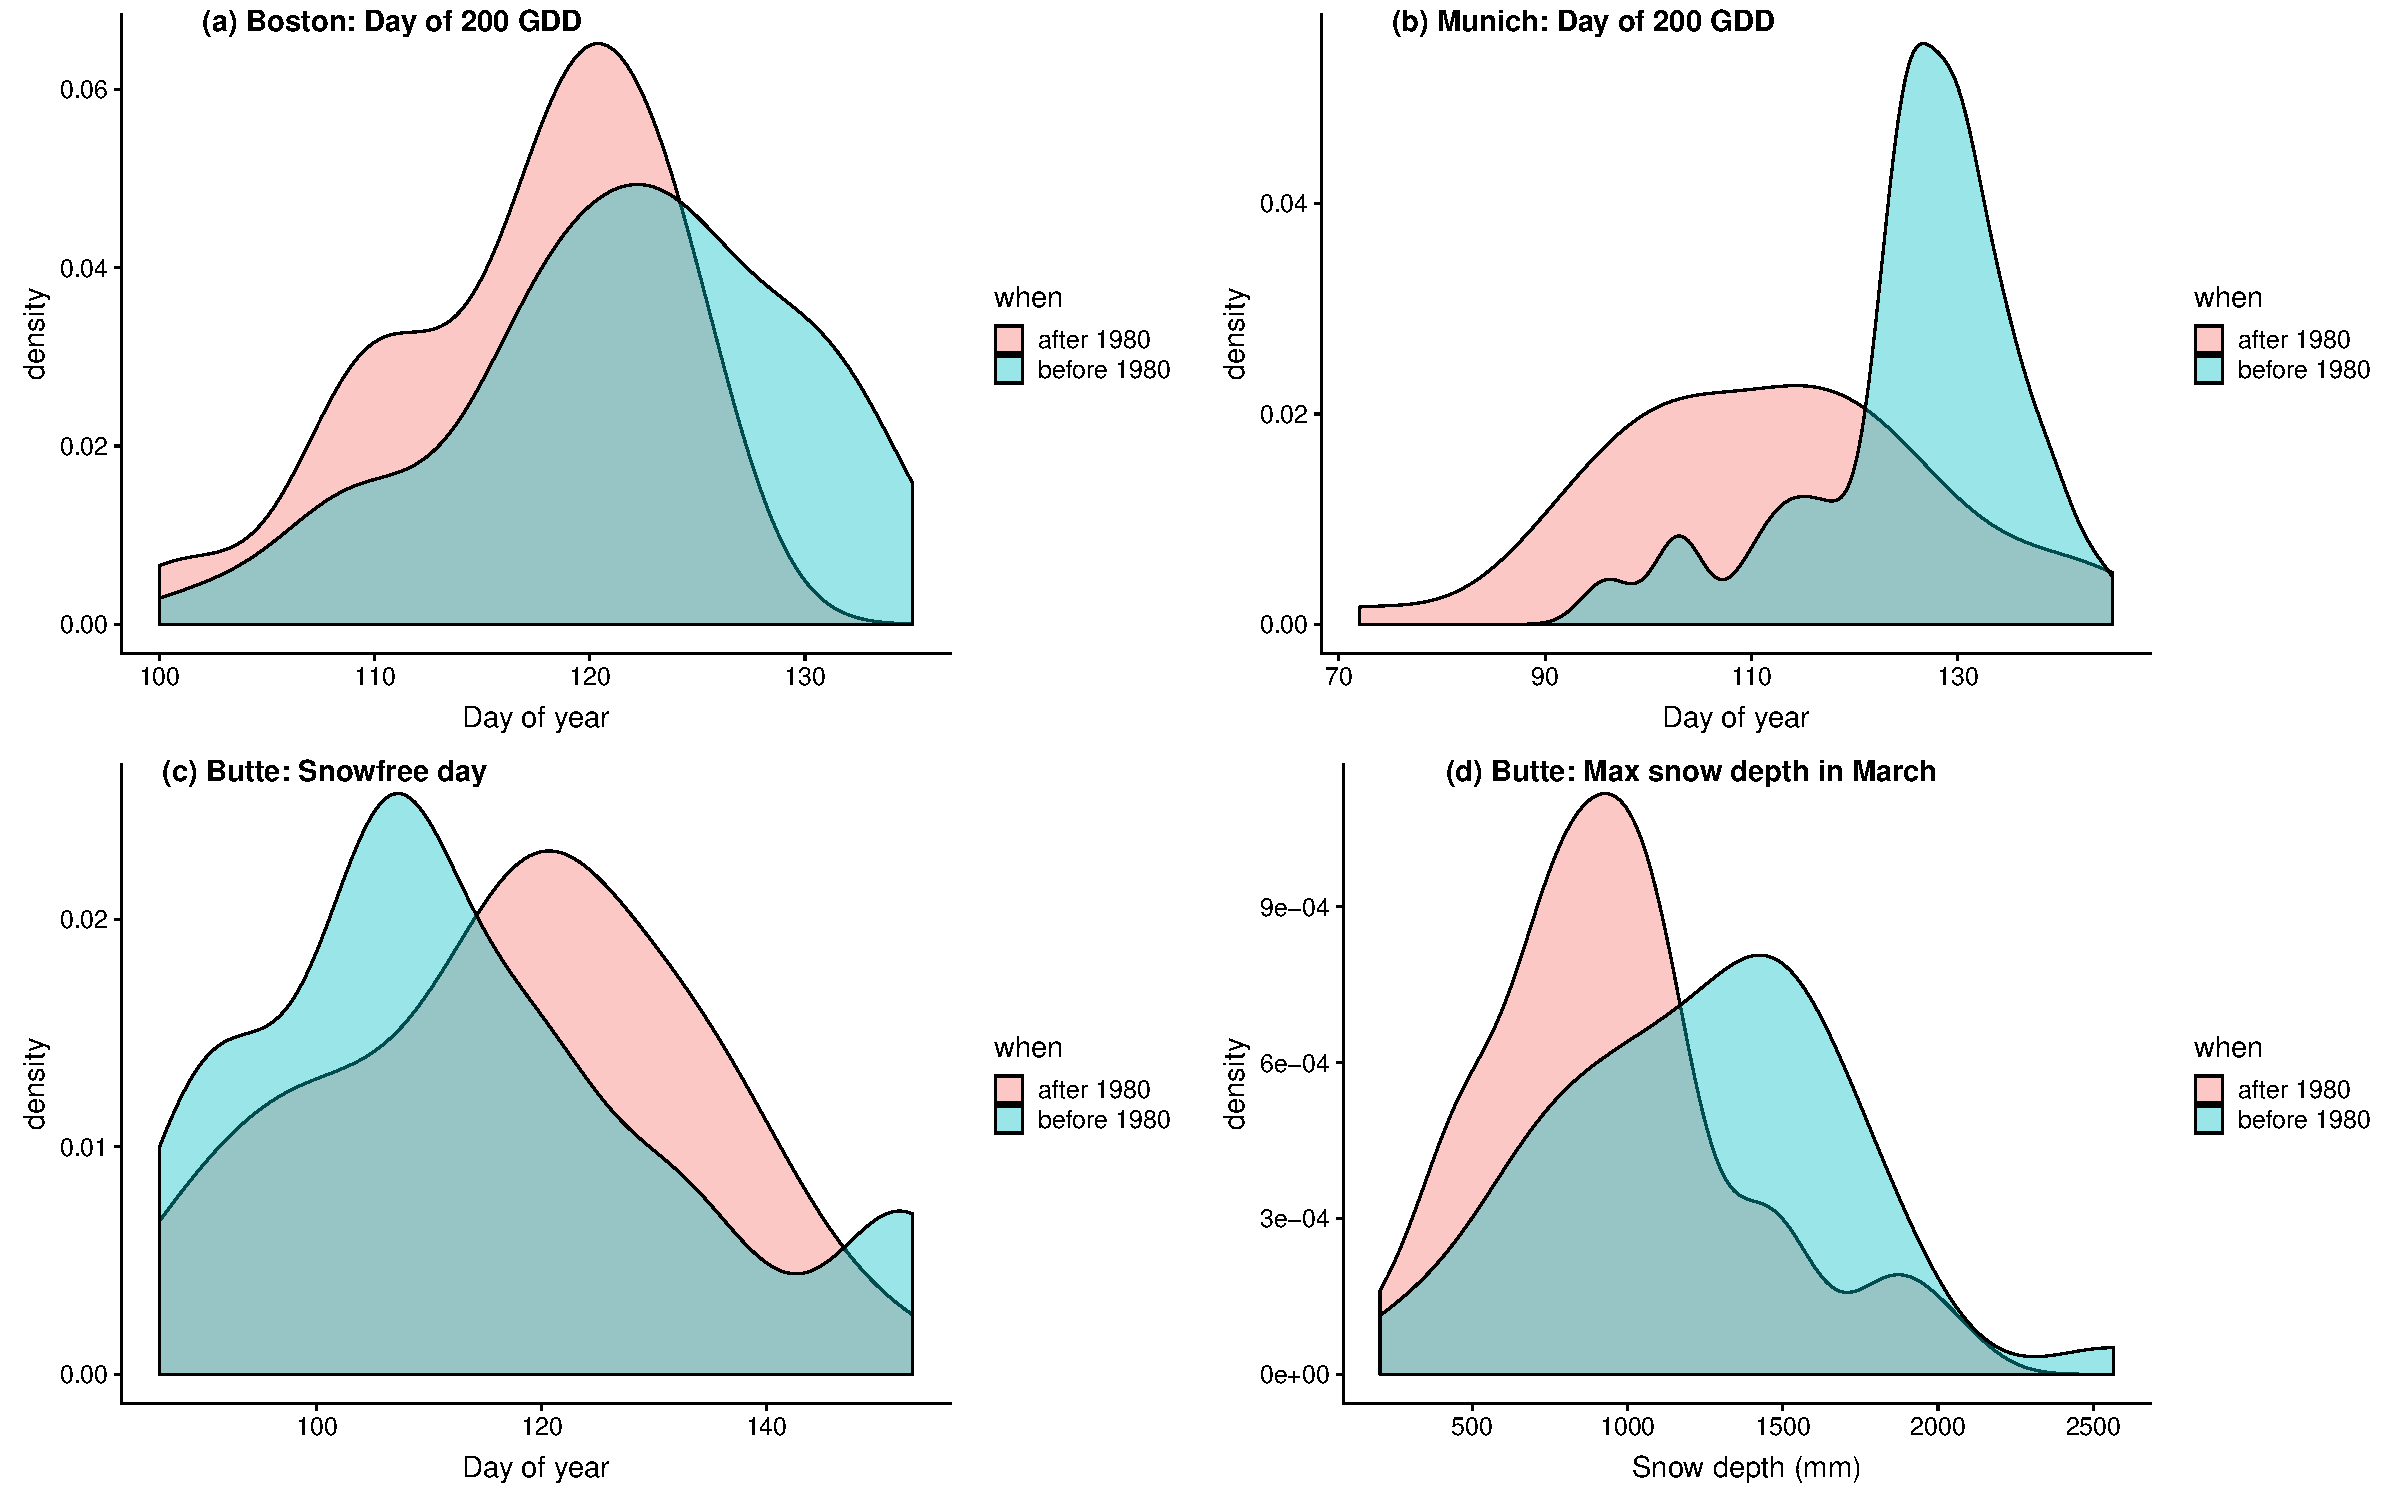
\includegraphics[width=1\textwidth]{..//..//..//R/graphs/otherdat/climdata.pdf}
\caption{Understanding non-stationarity in ecological systems requires first identifying which aspects of the environment have shifted---and how they have shifted with respect to one another \citep[e.g.,][]{cookwine2016,wadgymar2018}---as the underlying  distributions transition from stationary to non-stationary. Here we show examples of non-stationarity in climate variables that affect phenology by comparing before and after 1980 (a major change-point in climate for many regions) in several metrics related to the start of growing seasons (a-c) or resource pulse connected to growing season length (d). Density plots of day of 200 growing degree day units (a metric of thermal sum, here based on 0 degree base temperature using daily minima in $\degree$C) in Boston, MA, USA (a), and Munich, Germany (b), first snowfree day (followed by at least 9 snowfree days) in Crested Butte, CO, USA (c) and maximum snowdepth (mm) in March (often the month before the first snowfree day) in Crested Butte, CO, USA (d). Note that (c) and (d) are likely related, with lower snowpacks leading to an earlier first snowfree day. We selected sites that have been studied for plant phenological data and included at least 80 years of daily climate data from a Global Historical Climatology Network site; we subsetted data so that there were 40 years before and after 1980 for all sites.} %  (downloaded from \href{https://climexp.knmi.nl/})
% (Fig. \ref{fig:climdat}). For example, with climate change, warming has increased mean temperatures over time, with minimum temperatures generally increasing more than maximum---this results in an underlying distribution for daily temperature where the mean is increasing through time while the within-day variance is decreasing \citep{ipcc2013,screen2014}. Additionally, climate change has decoupled historical relationships between precipitation and temperature in some systems \citep[e.g.,][]{cookwine2016,wadgymar2018}. Understanding the impacts of climate change further requires recognizing that most systems can be considered stationary or non-stationary depending on the timescale and period of study. Thus, predicting the consequences of current non-stationarity in ecological systems benefits from identifying the type and scale of non-stationarity, relative to long-term trends. 
 \label{fig:climdat}
\end{figure}


\begin{figure}[h!]
\centering
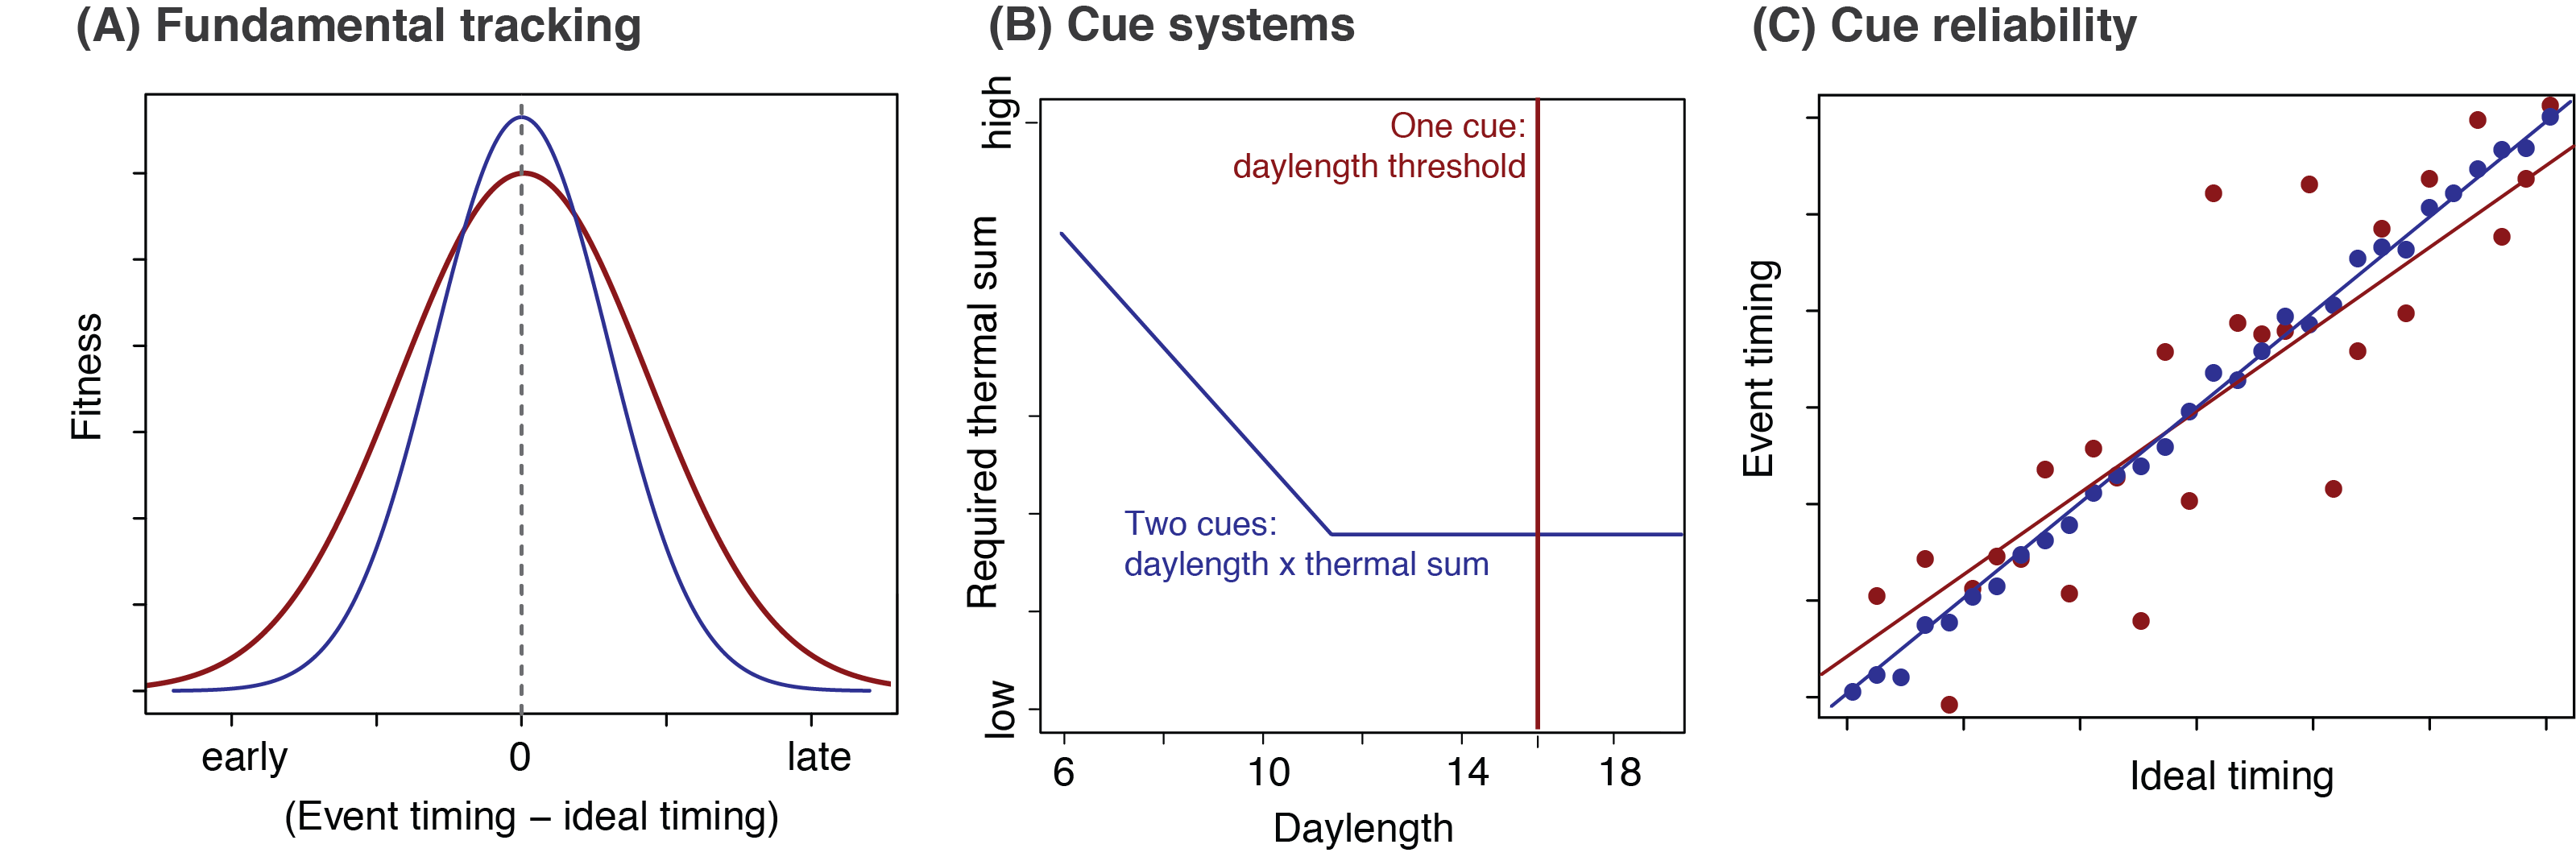
\includegraphics[width=1\textwidth]{..//..//..//R/graphs/conceptual/envtracking_define2.png}
\caption{Fundamental tracking (A) represents how an organism matches the actual timing of a life history event (phenology) to the timing that maximizes its fitness (i.e., ideal timing). Here, we show a common conceptualization where fitness declines as event timing moves away from the ideal timing, though realizations in nature may take diverse forms. As the ideal timing is generally only clear in simplified models or in retrospect, species that phenologically track must use a cue system (B) to try to match their phenology to the ideal timing across environments (temporally and/or spatially). Here we show two cue systems: one single cue system dependent only on daylength (red line: the event occurs when the organism's environment exceeds a certain daylength) and one multivariate cue system, which depends on a combination of daylength and thermal sums (navy line: the event occurs when the organism accumulates enough temperature for the current daylength). The match between ideal timing and actual timing represents cue reliability (C). } 
 \label{fig:defineETorig}
\end{figure}


\begin{figure}[h!]
\centering
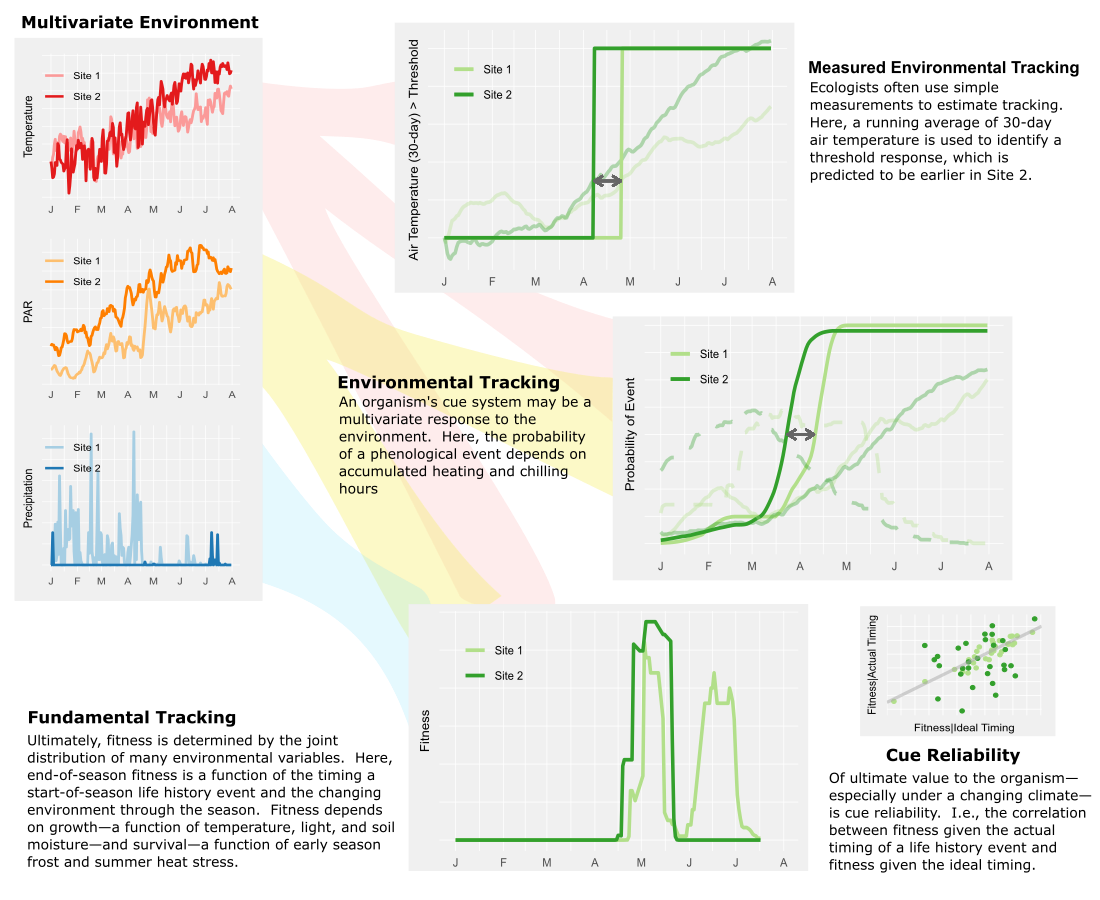
\includegraphics[width=1\textwidth]{..//..//..//R/graphs/conceptual/Fig3_pretty.png}
\caption{Dfferent components of a multivariate environment influence phenological tracking.  Ecologists may use a simple seasonal metric to \emph{measure environmental tracking}, but an organism's \emph{environmental tracking} may reflect more complex cues.  Ultimately, fitness is determined by the joint distribution of many environmental variables through time after the start-of-season life history event.  Cue reliability is the relationship between the timing that results from an organism's cue system and the fitness of the organism.  See SI `Fig. \ref{fig:defineET} methods' for further methods and details.} 
 \label{fig:defineET}
\end{figure}


\begin{figure}[h!]
\centering
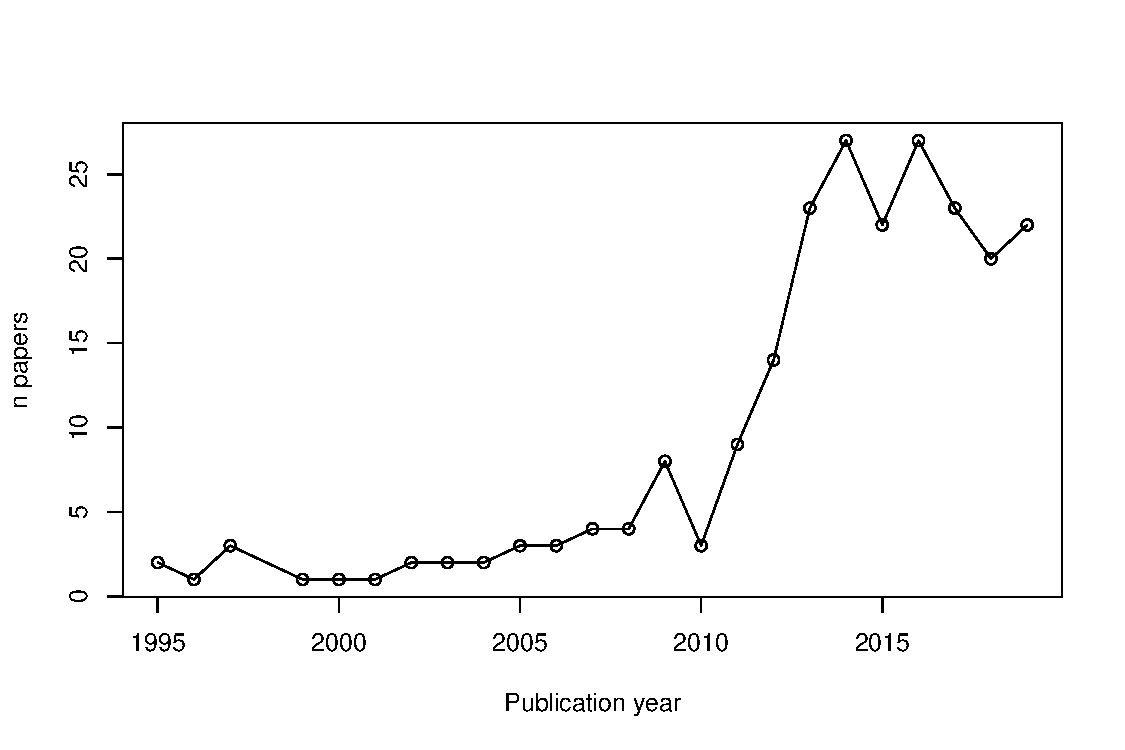
\includegraphics[width=0.9\textwidth]{..//..//..//R/graphs/otherdat/papersovertime.pdf}
\caption{Trends in all papers examining tracking \& other traits from a systematic literature review. We searched ISI (four searches: (1) Topic: `phenolog* chang*' and Title: phenolog* AND trait*, (2) Topic: `warming shift*' AND trait* and Title: phenolog*, (3) Topic: `phenolog* track*' AND trait* and Title: phenolog*, (4) Topic: `phenolog* sensitiv*' AND trait* and Title: phenolog*), which resulted in 231 papers, 83\% of which were published in 2011 or onward. Of papers from which we could extract data 25 of 30 were published in the same period. See SI, `Literature review of studies examining tracking \& other traits,' for detailed methods. }
  \label{fig:papertrends}
\end{figure}

\begin{figure}[h!]
\centering
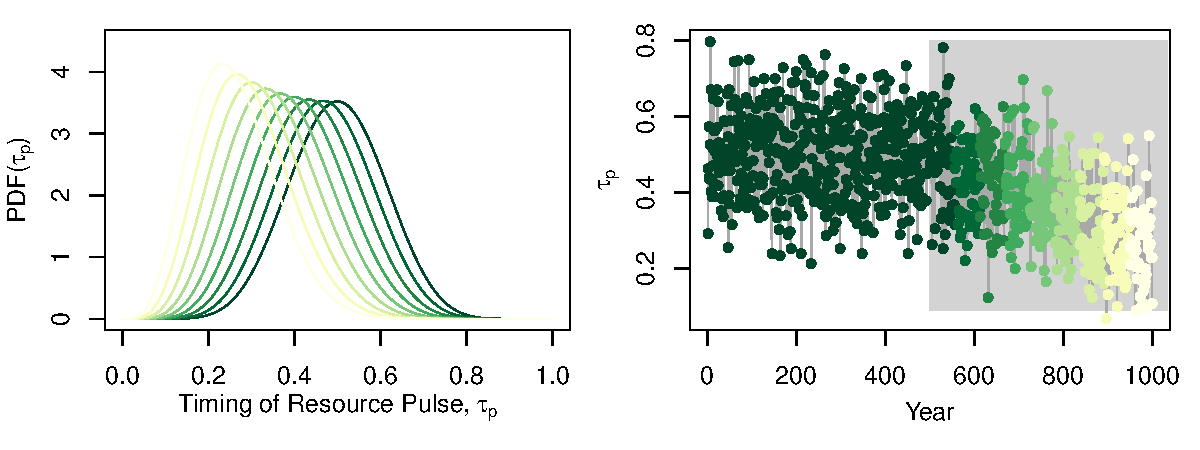
\includegraphics[width=1\textwidth]{..//..//..//R/graphs/modelruns/manuscript/modelsuppAlt.pdf}
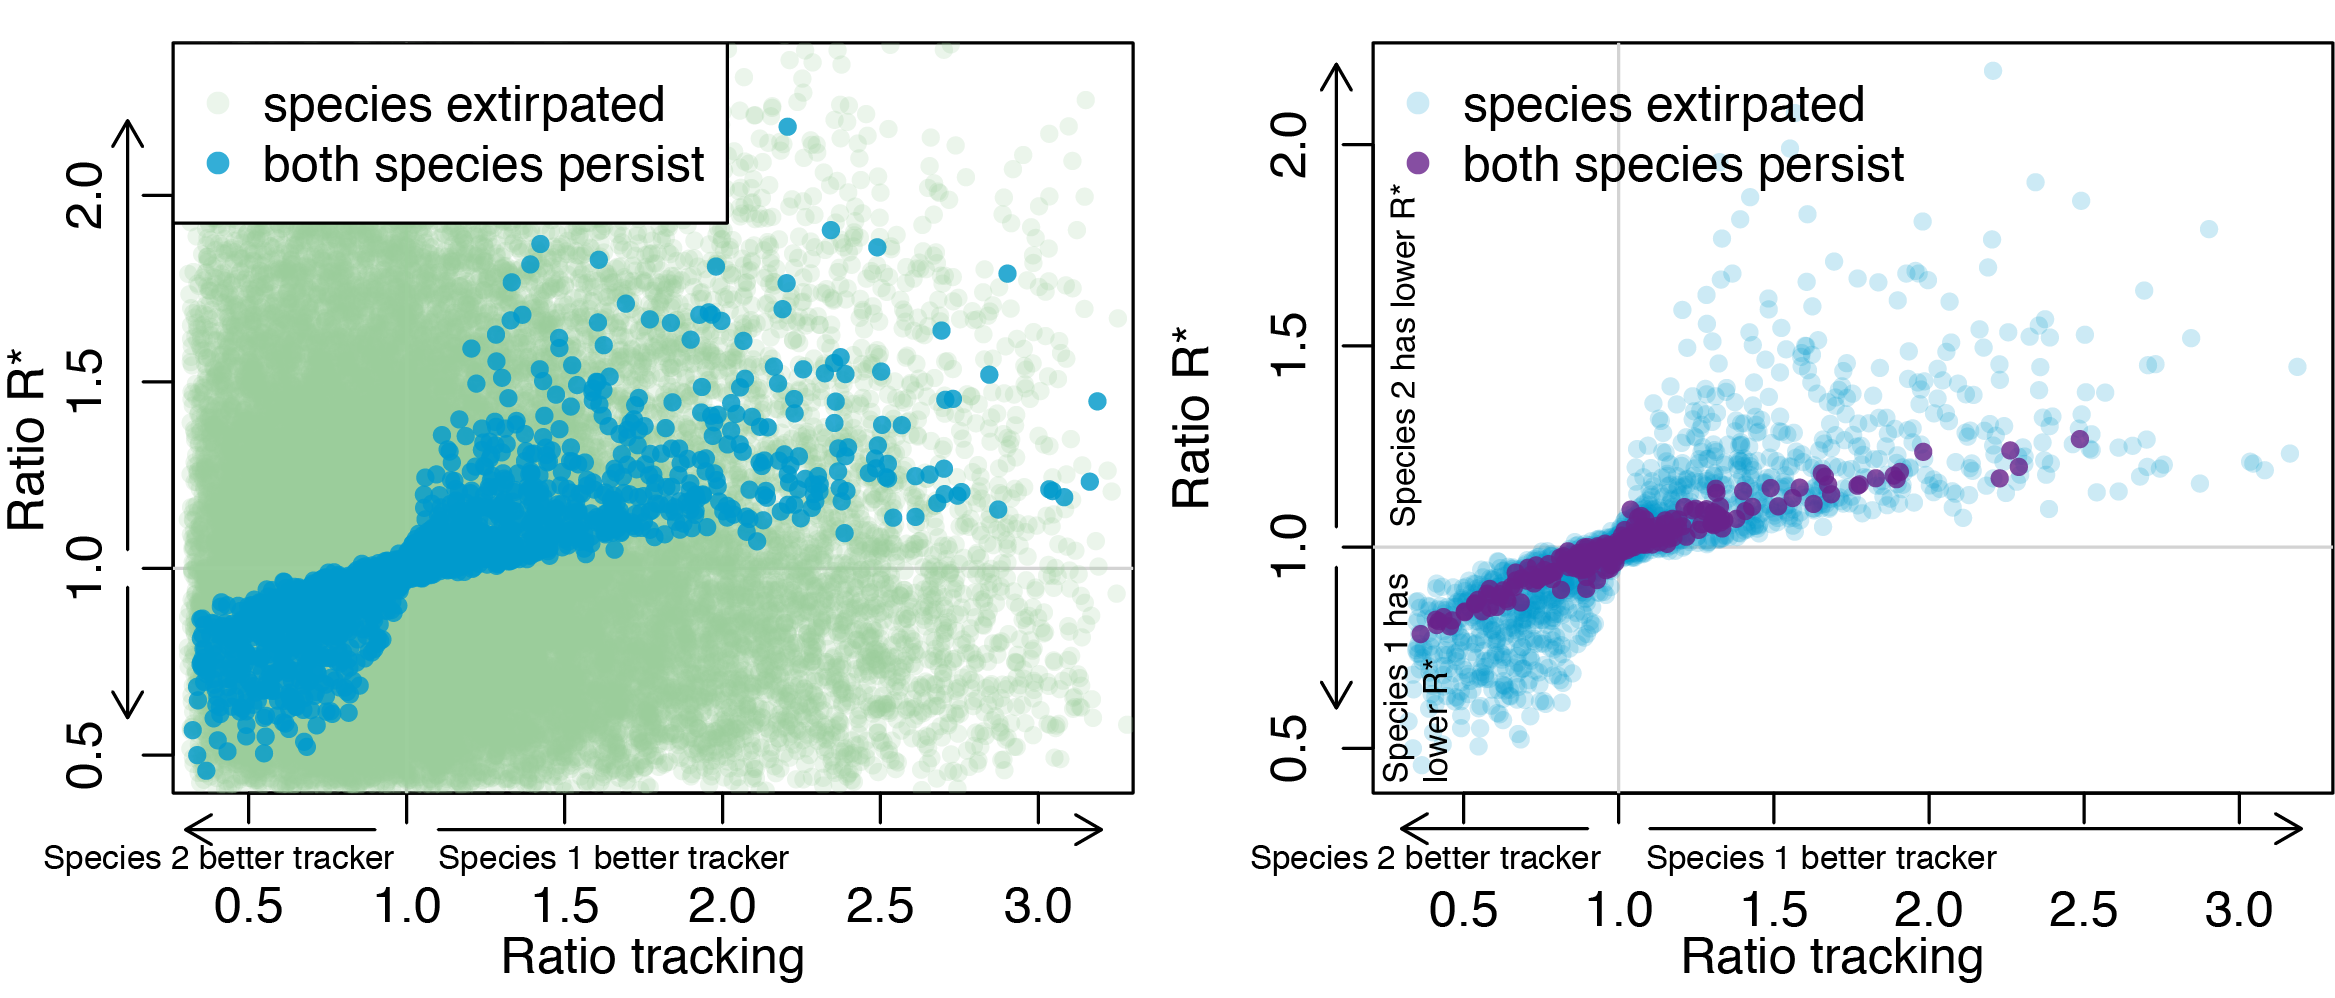
\includegraphics[width=0.96\textwidth]{..//..//..//R/graphs/modelruns/manuscript/alpharstar_2panelwide_adj.png}
\caption{Example of how non-stationarity can reshape communities in a simple coexistence model. We shifted the environment (top panels) by changing the timing of the resource pulse from a stationary period ($\tau_{p} \sim \beta(10,10)$ for the 500 years) to a nonstationary period ($\tau_{p}\sim \beta(5,15)$ over the 500 years), then examined outcomes for two-species communities (bottom panels) where tracking (X axis: species 1/species 2) trades off with $R^*$ (Y axis: species 1/species 2): each point represents one two-species community color-coded by whether both species persisted or one or more species was extirpated through 500 years of a stationary environment (bottom-left), followed by an additional 500 years of non-stationary environment (bottom-right, only two-species communities that persisted through the stationary period are shown).}
\label{fig:modelfig} 
\end{figure}

\begin{figure}[h!]
\centering
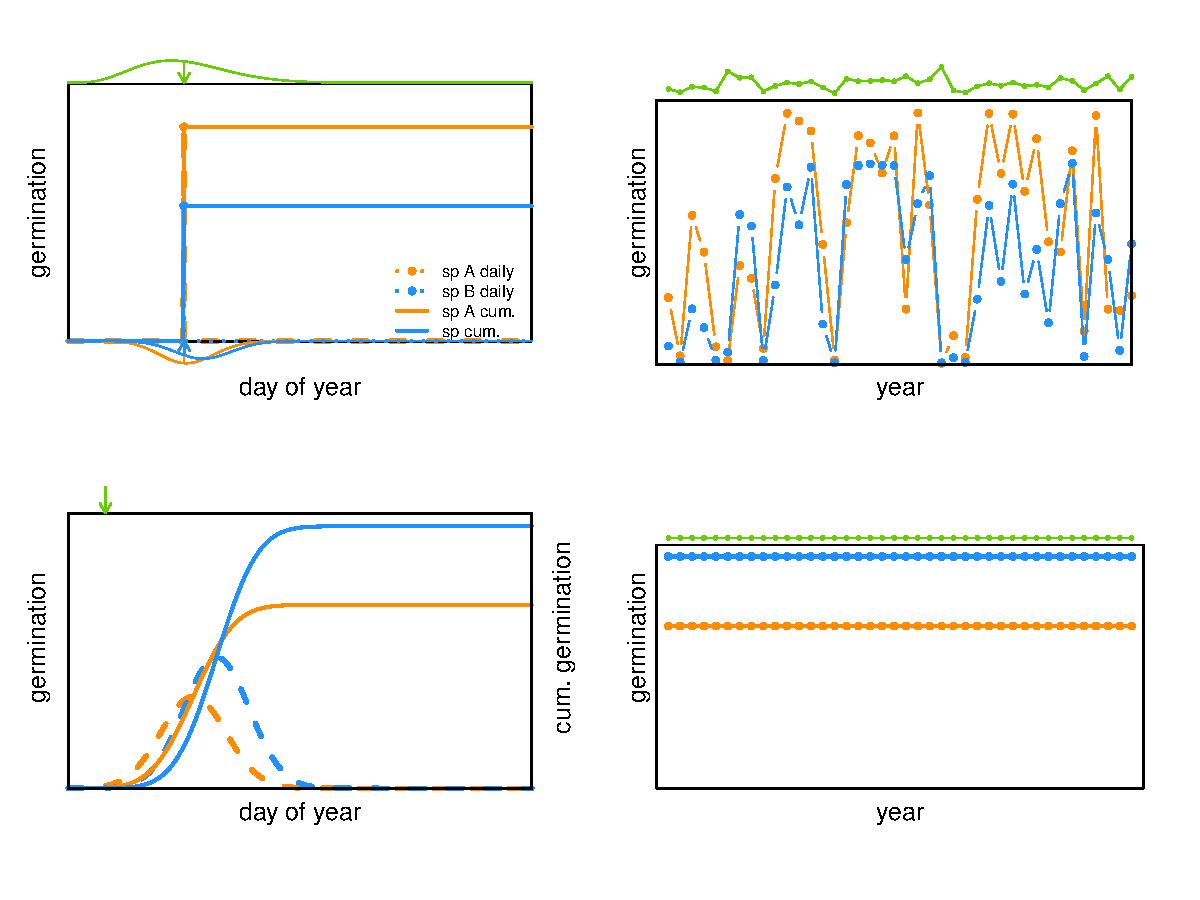
\includegraphics[width=1\textwidth]{..//..//..//R/graphs/conceptual/PriorityEff_BetHedge.pdf}
\caption{Tracking can be conceptualized as changes in priority effects or changes in storage effects.  In a priority effect model (A-B), the coexistence mechanism is a within-year tradeoff between, an early-germinating species that pre-empts resources (sp 1) and late-germinating species that is a superior resource competitor (sp 2) (A, where green arrow indicates the start of season); no between-year variation is required to maintain coexistence. In a storage effect model (C-D), variation in the timing of the start of season (indicated by the distribution in green, top of C) results results in differential species-response to the environment (illustrated by species-specific germination curves, bottom of C); this interannual variation in species-response to the environment (D)---along with a seedbank or other interannual storage mechanism---can maintain coexistence through reduced interspecific competition.}
\label{fig:conceptmodels} 
\end{figure}


%=======================================================================
% References
%=======================================================================
\clearpage
\newpage
% \section{References}
\bibliography{/Users/Lizzie/Documents/git/bibtex/LizzieMainMinimal}
\bibliographystyle{/Users/Lizzie/Documents/git/bibtex/styles/ecolett.bst}



%=======================================================================
% Tables
%=======================================================================

%\begin{center}  
%\begin{table}
%\caption{Key differences between PWR and traditional PCMs such as PGLS.}
%\begin{tabular}{ | p{4cm} | p{5.5 cm} | p{5.5 cm} |}   \hline 
%& PWR & PCMs (e.g., PGLS) \\ \hline \hline
%Major goal & Study of evolution of correlation between variables across species & Study of evolution of correlation between variables across species\\ \hline
%\emph{Assumption 1:} Nature of correlation between two or more variables & Non-stationary (changes through phylogeny in a phylogenetically conserved fashion) & Stationary (constant) throughout phylogeny (all variation is noise) \\ \hline
%\emph{Assumption 2:} Completeness of variables & Substitutes phylogeny for variables (simple or complex) not in the model that interact with variables in the model & Assumes variables in model are primary drivers of correlational relationship \\ \hline
%Inferential mode & Usually exploratory & Hypothesis testing (statistical significance)\\ \hline
%Outputs & Coefficients of regression changing through the phylogeny & p-value and single set of coefficients presumed to apply to entire phylogeny with their confidence intervals\\ \hline

%Method to avoid overfitting & Cross-validation (boot-strapped determination of optimal band-width for accurate prediction of hold-outs) & Exact analytical model of errors and degrees of freedom\\ \hline \hline
%\end{tabular}
%\end{table}
%\end{center}


\end{document}
%%%%%%%%%%%%%%%%%%%%%%%%%%%%%%%%%%%%%%%%%%%%%%%%%%%%%%%%%%%%%%%%%%%%%%%%


\emph{Box: Environmental variability \& change} 
Decades of ecological research highlight how temporally variable environments shape species and their communities at multiple scales \citep{Sale:1977oq,Chesson:1997dz}.  In seasonal landscapes, the environment limits periods for growth each year (e.g., by temperature, snowpack or drought); within-year variability in the environment (e.g., daily, hourly or finer resolution temperatures or rainfall amounts) compounds into inter-annual variability that shapes the distribution of the start and end of growing seasons. For long stretches of history this variability has been effectively stationary; that is, the underlying probability distribution that describes the start (or end) of the season (e.g., the date of the last major frost) does not change, even though the date may be dramatically different from one year to the  next. % The shape of this underlying distribution varies across systems and in how it is measured---for example, the total amount of rainfall across years in semi-arid systems is often highly skewed (rare high rainfall years, with many more below-average rainfall years) compared to the more normal (Gaussian) distribution of the thermal sum of temperate growing seasons. 
% In seasonal landscapes, periods for growth each year are limited (e.g., by temperature or drought), and species must manage within-year variability by timing when to grow and when to reproduce \citep{donohue2002}. 

In other time periods, variability has been non-stationary in one or multiple dimensions. For example, climate in the northern hemisphere includes long warming and then cooling periods (i.e., increasing then decreasing means of the probability distribution) at the start of the Holocene, when the earth was coming out of the last glacial maximum. Anthropogenic climate change is a similar non-stationary process, with warming evident around the globe and knock-on effects for other climate metrics, such as heat extremes and the size of precipitation events. % While only several decades ago, ecology was focused strongly on stochasticity in stationary systems \citep[e.g.,][]{Ripa1996,Kaitala1997}, climate change has shifted the focus to understanding stochasticity in a non-stationary framework \citep[e.g.,][]{cazwavelets,ehrlen2016,legault2019}.

Understanding non-stationarity in ecological systems requires first identifying which aspects of the environment have shifted---and how they have shifted with respect to one another---as the underlying  distributions transition from stationary to non-stationary (Fig. \ref{fig:climdat}). For example, with climate change, warming has increased mean temperatures over time, with minimum temperatures generally increasing more than maximum---this results in an underlying distribution for daily temperature where the mean is increasing through time while the within-day variance is decreasing \citep{ipcc2013,screen2014}. Additionally, climate change has decoupled historical relationships between precipitation and temperature in some systems \citep[e.g.,][]{cookwine2016,wadgymar2018}. Understanding the impacts of climate change further requires recognizing that most systems can be considered stationary or non-stationary depending on the timescale and period of study. Thus, predicting the consequences of current non-stationarity in ecological systems benefits from identifying the type and scale of non-stationarity, relative to long-term trends.  

% While most environments today are climatically non-stationary and have been for decades, the climate will return to a more stationarity form in the future. There are many possible pathways to climatic stabilization, but almost all require first the stabilization of greenhouse gases---the subject of much policy and political debate. Once greenhouse gas emissions stabilize climate will not quickly snap back to a new stationary phase. Instead systems will slowly approach a new climatic stationarity depending on how they are effected by the earth's multiple thermal reservoirs, and, in turn, how quickly those reservoirs stabilize. The timescale of this approach is generally expected to be on the scale of centuries, but could be much longer in certain oceanic systems \citep{ipcc2013ch12}. Thus, ecologists are---and will remain for the foreseeable future---in a research area structured by climatic non-stationarity. 



\begin{enumerate}
\item Figure for ... The shape of this underlying distribution varies across systems and in how it is measured---the amount of rainfall in semi-arid systems is often highly skewed compared the thermal sum of many temperate growing season
\item With climate change, warming has increased mean temperatures over time, with minimum temperatures generally increasing mre than maximum---this results in an underlying distribution for daily temperature where the mean is both increased through time and the variance is decreasing (Munich garden? Maybe add San Dieg precip example?
\item Real-world data showing stat/non-stationarity in environment (ideally $\tau_{p}$) 
\item Real-world data showing tracking (and less tracking)
\item $\tau_{i}$ vs. R* trade-off and histogram of persisting $\tau_i$ under stat/nonstat $\tau_{p}$ environment
\item alpha vs.$\tau_i$ trade-off and histogram of persisting alpha under stat/nonstat $\tau_{p}$ environment
\item alpha vs. R* trade-off and histogram of persisting alpha under stat/nonstat $\tau_{p}$ environment
\item (Scratch this one: we're pretty sure it required a crappy $\tau_i$ to survive the initial stationary period, then be favored in second time period and we're not so sure crappy $\tau_i$ species survive the initial stationary period) time-series of one run showing years where $\tau_i$ of one species is close to $\tau_{p}$ and other years where $\tau_i$ of other species is close to $\tau_{p}$ (and show this shift under nonstat)
\item non-stationarity in $R0$ and $\tau_{p}$
\end{enumerate}


%=======================================================================
% to-do listing
%=======================================================================

\listoftodos

%=======================================================================
\section*{Other loose ends}
%=======================================================================

% Old hypothesis: Without tracking we may predict benefits to early-colonizers decline with earlier seasons. As start-date moves earlier, early folks lose benefit (assuming they tend to often go at optimum time) and you get more late folks. Late species may be less different than one another---and less responsive to environment. Early folks, effectively, become more similar to environment. 

% Environmental variability means many species should benefit from tracking their environment. We focus here on environmental tracking through time (often referred to below as `tracking') rather than through space because of its well-established links to individual-level physiology, yielding a more robust understanding of what environmental cues determine tracking \citep{chuineJTB,Chew:2012pd}, and because it has been repeatedly linked to performance and other fitness-related metrics. Temporal environmental cues, however, are often linked to species' ranges \citep{Morin:2008vp,arabid2011}, thus we expect much of this work could extend to environmental tracking through space. 
% Definition of tracking: correlation between a recurring biological event and something else in its environment

Many (or potentially all) species use abiotic cues to trigger major phenological events. These cues in turn result in different rates of tracking. At one extreme, some cues yield a fixed timing, resulting in no tracking over time. A common example of a fixed cue is photoperiod, which results in event timing that is constant across years (but variable across space, allowing---for example, later timings poleward for spring events) and appears widespread for some insect emergence and for fall senescence of many trees \citep{Denlinger2017,lechowiczbook2002}. Fixed timings are perhaps the simplest option and may be efficient for events where there is low predictability, low variability, or low costs to being too late or early. In cases where there is a high cost to mis-timing an event across a variable environment, cues that yield more variability in timing are far more prevalent and usually rely on climate. Temperature is a widespread cue for start of season events with many organisms needing a certain thermal sum to start visible growth. Such a cue has the benefit of shifting the date of an event early or late, depending on climatic conditions, each year, but may be a poor cue in years with aberrant events (e.g., a late frost). In most systems, species must use environmental cues such as temperature to forecast the ideal date for an event---a date which is only obvious in retrospect. ...  Measuring tracking depends on many factors (see Box `What underlies variability in species tracking?'). 






